% ****** Start of file apssamp.tex ******
%
%   This file is part of the APS files in the REVTeX 4.2 distribution.
%   Version 4.2a of REVTeX, December 2014
%
%   Copyright (c) 2014 The American Physical Society.
%
%   See the REVTeX 4 README file for restrictions and more information.
%
% TeX'ing this file requires that you have AMS-LaTeX 2.0 installed
% as well as the rest of the prerequisites for REVTeX 4.2
%
% See the REVTeX 4 README file
% It also requires running BibTeX. The commands are as follows:
%
%  1)  latex apssamp.tex
%  2)  bibtex apssamp
%  3)  latex apssamp.tex
%  4)  latex apssamp.tex
%
\documentclass[%
 reprint,
%superscriptaddress,
%groupedaddress,
%unsortedaddress,
%runinaddress,
%frontmatterverbose, 
%preprint,
%preprintnumbers,
%nofootinbib,
%nobibnotes,
%bibnotes,
 amsmath,amssymb,
 aps,
%pra,
%prb,
%rmp,
%prstab,
%prstper,
%floatfix,
]{revtex4-2}
\usepackage{kotex}
\usepackage{graphicx}% Include figure files
\usepackage{dcolumn}% Align table columns on decimal point
\usepackage{bm}% bold math
\usepackage{tikz}
\usetikzlibrary{arrows}

% Nice captions.
\usepackage[hang,small,bf]{caption}
\setlength{\captionmargin}{25pt}

% New commands to keep things tidy.

%\usepackage{hyperref}% add hypertext capabilities
%\usepackage[mathlines]{lineno}% Enable numbering of text and display math
%\linenumbers\relax % Commence numbering lines

%\usepackage[showframe,%Uncomment any one of the following lines to test 
%%scale=0.7, marginratio={1:1, 2:3}, ignoreall,% default settings
%%text={7in,10in},centering,
%%margin=1.5in,
%%total={6.5in,8.75in}, top=1.2in, left=0.9in, includefoot,
%%height=10in,a5paper,hmargin={3cm,0.8in},
%]{geometry}

\def\rcurs{{\mbox{$\resizebox{.16in}{.08in}{\includegraphics{ScriptR}}$}}}
\def\brcurs{{\mbox{$\resizebox{.16in}{.08in}{\includegraphics{BoldR}}$}}}
\def\hrcurs{{\mbox{$\hat \brcurs$}}}

\begin{document}


\title{리드베리 상수 측정 실험 보고서}

\author{서울대학교 전기정보공학부 2018-12432 박정현}
 \email{alexist@snu.ac.kr}
\date{\today}% It is always \today, today,
             %  but any date may be explicitly specified

\begin{abstract}
Abstract
\end{abstract}

%\keywords{Suggested keywords}%Use showkeys class option if keyword
                              %display desired
\maketitle

%\tableofcontents

\section{\label{sec:level1}Introudction}
\subsection{\label{sec:level2}방전관}
유전체 양단에 강한 전압을 인가하면 절연파괴 현상이 일어난다. 이때 방전관 내부에 있는 원자들이 전자들을 흡수, 방출하면서 방전관 외부로 광자를 방출하게 된다. 이 때 광자는 원자들의 에너지 준위 차이에 해당하는 주파수를 가진다. 이러한 주파수, 혹은 파장에 따른 스펙트럼을 확인하면 원자의 에너지 준위를 분석할 수 있다.

\subsection{\label{sec:level2}스펙트럼}
원자 내부에는 다양한 에너지 레벨이 존재한다. 이러한 에너지 레벨이 충분히 멀리 떨어져 있는 경고 입사하는 광자의 에너지가 해당 에너지레벨 차이에 가까운 경우 2 level system으로 근사할 수 있다. Ground state, 그리고 상호작용하는 enery level을 모두 고려하면 Fig.\label{fig:Level}과 같이 에너지 레벨을 나타낼 수 있다. 이 때 외부로부터 excite되는 원자들의 비율이 $\Lambda$라고 할 때 아래의 식이 성립한다. 단, $\rho_{nm}$은 photon state $nm$에 대한 density matrix에 해당한다.

\begin{figure}
\centerline{
  \resizebox{8cm}{!}{
    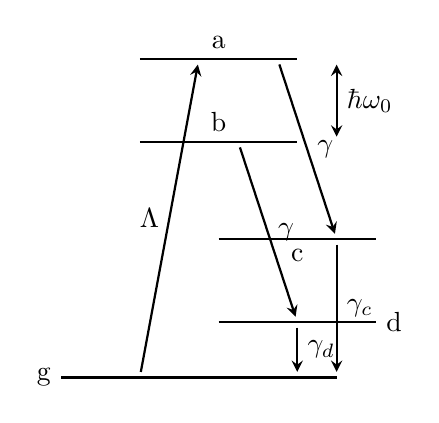
\begin{tikzpicture}[
      scale=0.5,
      level/.style={thick},
      virtual/.style={thick,densely dashed},
      trans/.style={thick,->,shorten >=2pt,shorten <=2pt,>=stealth},
      trans2/.style={thick,<->,shorten >=2pt,shorten <=2pt,>=stealth},
      classical/.style={thin,double,<->,shorten >=4pt,shorten <=4pt,>=stealth}
    ]
    % Draw the energy levels.
    \draw[level] (6cm,-12em) -- (-1cm,-12em) node[left] {g};
    \draw[level] (1cm,11em) -- (5cm,11em) node[midway,above] {a};
    \draw[level] (3cm,-8em) -- (7cm,-8em) node[right] {d};
    % Draw the virtual levels.
    \draw[level] (1cm,5em) -- (5cm,5em) node[midway,above] {b};
    \draw[level] (3cm,-2em) -- (7cm,-2em) node[midway,below] {c};
    % Draw the transitions.
    \draw[trans] (1cm,-12em) -- (2.5cm,11em) node[midway,left] {$\Lambda$};
    \draw[trans2] (6cm,5em) -- (6cm,11em) node[midway,right] {$\hbar \omega_{0}$};
    \draw[trans] (3.5cm,5em) -- (5cm,-8em) node[midway,right] {$\gamma$};
    \draw[trans] (4.5cm,11em) -- (6cm,-2em) node[midway,right] {$\gamma$};
    \draw[trans] (5cm,-8em) -- (5cm,-12em) node[midway,right] {$\gamma_{d}$};
    \draw[trans] (6cm,-2em) -- (6cm,-12em) node[midway,right] {$\gamma_{c}$};
    \end{tikzpicture}
  }
}
\caption{\label{fig:Level}방전관에서 광자 방출 diagram}
\end{figure}

\begin{align}
	\dot{\rho}_{nm} &= -\frac{i}{\hbar}\text{Tr}_{atom}[H_{I},\rho]_{nm} + (L\rho)_{nm}
\end{align}

위의 식을 정리하면 아래와 같아진다.

\begin{align}
	\begin{split}
	\dot{\rho}_{nm} &= -\left(\frac{N_{nm}'G}{1+N_{nm}S/G}\right)\rho_{nm} \\
	& + \left(\frac{\sqrt{nm} G}{1+N_{n-1,m-1}S/G}\right)\rho_{n-1,m-1} \\
	& - \kappa(n+m)\rho_{nm} \\
	& + 2\kappa\sqrt{(n+1)(n+1)}\rho_{(n+1)(m+1)}
	\end{split}
\end{align}

단, 상수들은 아래와 같다.

\begin{align}
	G &= N\frac{\Lambda}{\gamma + \Lambda} \frac{2g^{2}}{\gamma} \\
	S &= \frac{4g^{2}}{\gamma^{2}}G\\
	N_{nm}' &= \frac{1}{2}(n+1+m+1) + \frac{(n-m)^{2}S}{8G}\\
	N_{nm} &= \frac{1}{2}(n+1+m+1) + \frac{(n-m)^{2}S}{16G}
\end{align}

$n=m$인 경우만 고려하면 $\rho_{nm} = p(n)$에 해당한다. $S\langle n \rangle / G \gg 1$인 경우를 고려하면 평균 광자수 $\langle n \rangle$ 은 아래와 같아진다.
\begin{align}
	\langle n \rangle &\simeq \frac{G}{2\kappa}\left( \frac{G-2\kappa}{S} \right)\\
	&\simeq N\frac{\Lambda}{\gamma + \Lambda} \frac{2g^{2}}{2\kappa\gamma} \frac{\gamma^{2}}{4g^{2}}\\
	& \simeq N\frac{\gamma}{4\kappa}
\end{align}

광자의 방출을 random event로 고려하는 경우 line width는 아래와 같아진다.

\begin{align}
	\Delta \omega \simeq \frac{2\kappa}{\langle n \rangle}
\end{align}

Spontaneous decay rate만을 고려하면 $\gamma$는 아래와 같아진다.
\begin{align}
	\gamma \simeq \frac{2e^{2}\omega_{0}^{2}}{3mc^{2}}
\end{align}

따라서 에너지 사이의 간격 $\omega_{0}$가 커지는 경우 $\gamma$가 증가하므로 평균 광자수가 증가한다. 또한 평균 광자수가 증가하므로 line width는 이에 비례하여 작아지게 된다.

\section{\label{sec:level1}Reference}
[1] S.M. Sze, Y. Li, and K.K. Ng, \textit{Physics of Semiconductor Devices} (Wiley-Interscience, Hoboken, , 2021). 

[2] Griffiths, \textit{Introduction to Electrodynamics} (Cambridge University Press, 2017). 

[3] D. Halliday, R. Resnick, J. Walker, and S.-B. Liao, \textit{Fundamentals of Physics} (Wiley, Hoboken, NJ, 2013). 

\end{document}
%
% ****** End of file apssamp.tex ******
